
\documentclass[runningheads,a4paper]{llncs}

\usepackage[ngerman]{babel}

\usepackage{graphicx}
\usepackage[table]{xcolor}

\usepackage{wrapfig}

%extended enumerate, such as \begin{compactenum}
\usepackage{paralist}

%put\ figures\ inside\ a\ text
%\usepackage{picins}
%use
%\piccaptioninside
%\piccaption{...}
%\parpic[r]{\includegraphics ...}
%Text...

%Sorts the citations in the brackets
%\usepackage{cite}

%for easy quotations: \enquote{text}
\usepackage{csquotes}

\usepackage[T1]{fontenc}
\usepackage[utf8]{inputenc}

%enable margin kerning
\usepackage{microtype}

%better font, similar to the default springer font
\usepackage[%
rm={oldstyle=false,proportional=true},%
sf={oldstyle=false,proportional=true},%
tt={oldstyle=false,proportional=true,variable=true},%
qt=false%
]{cfr-lm}
%
%if more space is needed, exchange cfr-lm by mathptmx
%\usepackage{mathptmx}


\usepackage[
	%pdfauthor={},
	%pdfsubject={},
	%pdftitle={},
	%pdfkeywords={},
	bookmarks=false,
	breaklinks=true,
	colorlinks=true,
	linkcolor=black,
	citecolor=black,
	urlcolor=black,
	%pdfstartpage=19,
	pdfpagelayout=SinglePage
]{hyperref}

%enables correct jumping to figures when referencing
\usepackage[all]{hypcap}

\usepackage[capitalise,nameinlink]{cleveref}
%Nice formats for \cref
\crefname{section}{Abschnitt}{Abschnitte}
\Crefname{section}{Abschnitt}{Abschnitte}
\crefname{figure}{Abb.}{Abb.}
\Crefname{figure}{Abbildung}{Abbildungen}

\usepackage{xspace}
%\newcommand{\eg}{e.\,g.\xspace}
%\newcommand{\ie}{i.\,e.\xspace}
\newcommand{\eg}{e.\,g.,\ }
\newcommand{\ie}{i.\,e.,\ }

%introduce \powerset - hint by http://matheplanet.com/matheplanet/nuke/html/viewtopic.php?topic=136492&post_id=997377
\DeclareFontFamily{U}{MnSymbolC}{}
\DeclareSymbolFont{MnSyC}{U}{MnSymbolC}{m}{n}
\DeclareFontShape{U}{MnSymbolC}{m}{n}{
    <-6>  MnSymbolC5
   <6-7>  MnSymbolC6
   <7-8>  MnSymbolC7
   <8-9>  MnSymbolC8
   <9-10> MnSymbolC9
  <10-12> MnSymbolC10
  <12->   MnSymbolC12%
}{}
\DeclareMathSymbol{\powerset}{\mathord}{MnSyC}{180}

%improve wrapping of URLs - hint by http://tex.stackexchange.com/a/10419/9075
\makeatletter
\g@addto@macro{\UrlBreaks}{\UrlOrds}
\makeatother

% correct bad hyphenation here
\hyphenation{op-tical net-works semi-conduc-tor}


\def\dcn{\colorbox{yellow}{$^{\texttt{Zitat benötigt}}$}~}

\begin{document}

%Works on MiKTeX only
%hint by http://goemonx.blogspot.de/2012/01/pdflatex-ligaturen-und-copynpaste.html
%also http://tex.stackexchange.com/questions/4397/make-ligatures-in-linux-libertine-copyable-and-searchable
%This allows a copy'n'paste of the text from the paper
\input glyphtounicode.tex
\pdfgentounicode=1

\title{Web Technologien: Ransomware}
%If Title is too long, use \titlerunning
\titlerunning{Web Technologien: Ransomware}

%Single insitute
\author{Abwandner, Sebastian und Beham, Michael und Schmid, Pascal}
%If there are too many authors, use \authorrunning
\authorrunning{HSA - Abwandner, Beham, Schmid}
\institute{
	Hochschule Augsburg \\
	An der Hochschule 1 \\
	86161 Augsburg
}


\maketitle

\begin{abstract}
Die letzten Jahre haben gezeigt, dass Ransomware nicht nur für die IT-Sicherheit zum immer größer werdenden Problem wird. Obwohl schon vor Jahrzehnten die erste Ransomware entdeckt wurde, ist es durch anonyme Zahlungsmethoden des Internets für Angreifer einfacher geworden Geld mit Malware zu verdienen. Diese Arbeit gibt einen Überblick über die Entwicklungen der letzten Jahre, die Ransomware-Angriffe im großen Stil möglich machten, über die technische Funktionsweise, psychologische Hintergründe und mögliche Gegenmaßnahmen. Zum Schluss lässt ein Ausblick in die Zukunft nochmals deutlich werden, welche Gefahren von Ransomware in den nächsten Jahren ausgehen.
\end{abstract}

%%%%%%%%%%%%%%%%%%%%%%%%%%%%%%%%%%%%%%%%%%%%%%%%%%%%%%%%%%%%%%%%%%%%%%%%%%%%%%%
\section{Einleitung}\label{sec:intro}
In den letzten Jahren haben sich die bekannt gewordenen Fälle von Ransomware vervielfacht.\dcn Waren früher noch irreführende Apps der Hauptanteil der Malware, wurde 2012 mit den sogenannten Lockern erstmals Malware entdeckt, die großflächig die betroffenen Anwender zur Bezahlung einer Lösegeldsumme veranlasst hat.\dcn In den Jahren 2014 und 2015 wurden diese eher harmlosen Varianten, die nur die Benutzung des Geräts blockiert haben, durch Crypto-Ransomware abgelöst. Diese verschlüsselt die Dateien des Benutzers und fordert zum Wiedererhalt eine Lösegeldsumme, die nicht-verfolgbar bezahlt werden soll. Schätzungen zufolge erbeuten die Hersteller von Crypto-Ransomware auf diesem Wege ca. 100 Millionen Euro pro Jahr. \cite{money}

	\begin{figure}[h!]
		\centering
		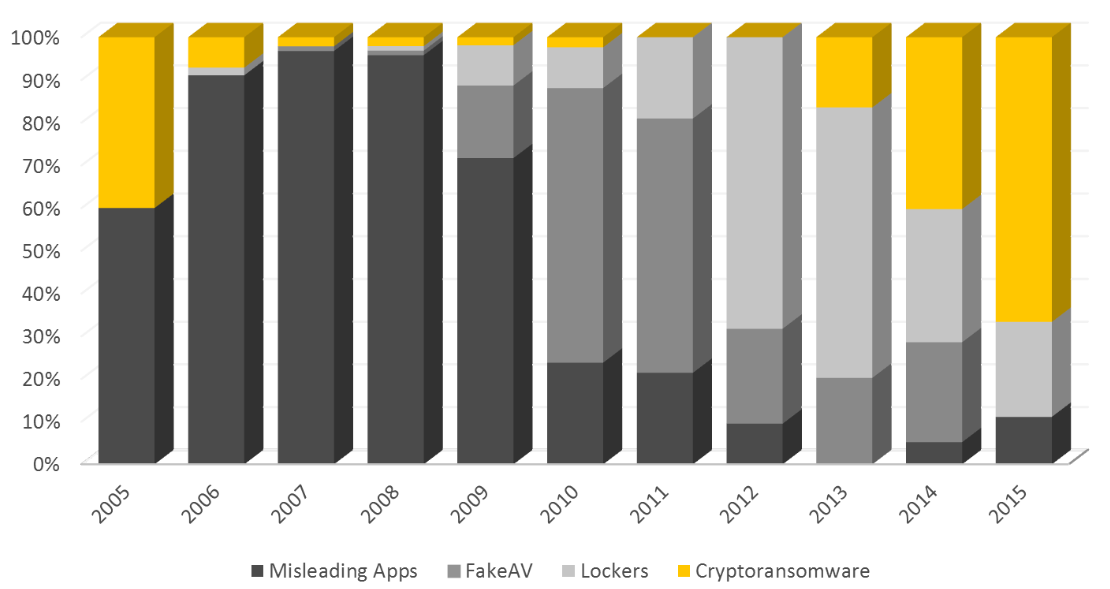
\includegraphics[width=\linewidth]{img/ransom-evolution.png}
		\caption{Evolution Malware Quelle: \cite{evolution}}
		\label{fig:ransom-evo}
	\end{figure}
%%%%%%%%%%%%%%%%%%%%%%%%%%%%%%%%%%%%%%%%%%%%%%%%%%%%%%%%%%%%%%%%%%%%%%%%%%%%%%%

\section{Kategorisierung}
Aufgrund der sich teilweise überschneidenden Funktionen im Bereich der Malware und der teils sehr unscharfen oder auch falschen Verwendung der Worte in Medien aller Art ist es schwierig eine allgemeingültige Definition dafür anzugeben. Im Rahmen dieser Arbeit wird sich jedoch an die Definitionen des Microsoft Protection Centers \cite{malware_pc} gehalten.

		\begin{itemize}
			\item \textbf{Bot:} Ein kleines, verstecktes Programm auf dem Rechner des Benutzers, oftmals vom Angreifer kontrolliert. Mehrere Bots, die über das Internet verbunden sind, nennt man ein Botnetz.
			\item \textbf{Botnetz:} Mehrere Kopien des­sel­ben Bots sind auf mehreren Rechnern installiert und werden von einem Angreifer kontrolliert. Mehrere Bots auf einer großen Anzahl infizierter Rechner nennt man Botnetz.
			\item \textbf{Malware:}	Kurzform für \glqq malicious software\grqq. Überbegriff für Software, die ungewollte Aktivitäten auf einem Rechner durchführt, wie etwa Daten stehlen, Dateien verschlüsseln oder Spam verschickt.
			\item \textbf{Ransomware:} Eine Art Malware, die den Benutzer daran hindert, das Gerät zu benutzen oder die Dateien verschlüsselt. Der Benutzer wird darüber informiert, dass er Geld bezahlen, eine Befragung oder eine sonstige Aktion durchführen muss, bevor er die Kontrolle wiedererlangt.
			\item \textbf{Trojaner:} Nach dem Trojanischen Pferd aus der Sage benannt, verhält sich diese Art von Malware unauffällig, um nicht entdeckt zu werden. Im Gegensatz zu Würmern oder Viren verbreitet sich ein Trojaner nicht von selbst weiter, sondern täuscht den Benutzer, um von diesem heruntergeladen oder installiert zu werden.
			\item \textbf{Virus:} Malware, die sich selbst weiterverbreitet, indem es reguläre Programme befällt und sich auf andere Systeme und Netzwerke weiterverbreitet.
			\item \textbf{Wurm:} Ein Wurm unterscheidet sich vom Virus dadurch, dass er mithilfe eines Trägers verbreitet wird. Dies kann etwa durch E-Mails, Instant Messaging, File-Sharing, Netzwerklaufwerke, Wechsellaufwerke und Ähnliches geschehen.
		\end{itemize}
Diese Einteilung gibt einen kurzen Überblick über die gebräuchlichsten Begrifflichkeiten, ist aber nicht abschließend. \\
Einer klaren Kategorisierung steht auch entgegen, dass Schädlinge meist in mehrere Kategorien fallen und sich diese auch teilweise überschneiden.

\section{Aktuelle Ransomware}
Alle hier beschriebenen Ransomware sind innerhalb der letzten Jahre erschienen und beschreiben somit den zum Schreiben des vorliegenden Papers aktuellen Stand der Technik.

\subsection{TeslaCrypt}
TeslaCrypt war der erste der modernen Crypto-Ransomware, der von den Medien aufgegriffen wurde und somit einer breiten Öffentlichkeit bekannt gemacht wurde. Ende 2015 \cite{tesla:entdeckt} wurde dieser entdeckt, jedoch wurde bereits kurze Zeit später ein Tool veröffentlicht \cite{tesla:geknackt}, mit dem betroffene Anwender ihre Daten retten konnten.

Version 3 der Ransomware wurde von den Angreifern grundlegend verändert. So wurde der Algorithmus zum Schlüsselaustausch erneuert, was es vorerst unmöglich gemacht hat, den privaten Schlüssel der Ransomware aus den verschlüsselten Dateien abzuleiten. \cite{tesla:version3} \cite{tesla:version3_2}

Version 4 kann zudem Dateien größer als 4 GB verschlüsseln \cite{tesla:version4}, zuvor wurden Dateien größer als dieses Limit unwiderruflich zerstört. In der vorerst letzten veröffentlichen Version 4.1a \cite{tesla:version41} wurden weitere Dateitypen verschlüsselt. So wurden unter anderem Bitcoin-Wallets und Spielstände verschlüsselt, die für den Nutzer ein angenommenen materiellen und auch ideellen Wert haben.

Am 18. Mai 2016 wurde bekannt, dass die Entwickler von TeslaCrypt die Weiterentwicklung eingestellt haben und als Entschuldigung den Schlüssel zur Verschlüsselung frei auf ihrer Webseite veröffentlicht haben. Die Wochen zuvor wurde von Experten der IT-Sicherheitsfirma ESET bereits festgestellt, dass die Entwickler der Ransomware ihre Aktivitäten immer weiter verringern. \cite{tesla:end}

\subsection{Locky}
Anfang 2016 wurde eine neue Ransomware entdeckt, die aufgrund der Dateiendung der verschlüsselten Daten in den Medien als \glqq Locky\grqq{} bekannt wurde. Es wurden nicht nur Bilder, Dokumente, Videos und Musik angegriffen, sondern zudem auch Datenbanken, Quellcode, Zertifikate und Krypto-Schlüssel. Durch die lange Liste an angegriffenen Dateien rechnen die Entwickler von Locky mit einer höheren Chance, dass die betroffenen Anwender bereit sind, für den Wiedererhalt ihrer Dateien zu zahlen.

Die erste Welle des Angriffs wurde koordiniert zum gleichen Zeitpunkt gestartet, während sich Locky bis dahin noch im Netzwerk der befallenen Rechner verbreitet hat, um so möglichst viel Schaden auf einmal anzurichten. Die koordinierte Attacke zu einem Zeitpunkt hat es Administratoren verhindert etwa Netzwerksegmente bei seltsamen Aktivitäten von anderen abzuschotten, um so eine weitere Verbreitung zu verhindern. Locky hat des Weiteren noch Windows-Schattenkopien gelöscht, mit denen ein Wiederherstellen der verschlüsselten Dateien möglich gewesen wäre. \cite{locky:start}

Die Infizierung der Rechner erfolgte anfangs mit einem Microsoft Office-Dokument, in dem Makros enthalten waren \cite{locky:infection}. Das Dokument selbst war unleserlich, ähnlich einer fehlerhaften Zeichensatz-Decodierung. Am Anfang des Dokuments stand der Hinweis, dass falls das Dokument unleserlich sei, der Nutzer die Verwendung von Makros einschalten sollte. Hierdurch wurde schließlich die Infizierung ermöglicht.

Kurze Zeit später wurde bekannt, dass die Infizierung auch auf weiteren Wegen erfolgt: Als Erstes wurde per angeblichem Fax von einem Fax-zu-E-Mail-Gateway eine Verbreitung erreicht \cite{locky:fax}, gefolgt von Windows-Batch-Dateien \cite{locky:batch}. Die verschiedenen Verbreitungskanäle der Ransomware und deren Fähigkeit durch die Verwendung von Skriptsprachen (Batch, Windows Script Host) mit der Möglichkeit, den Quelltext maschinell und leicht abzuändern und zu verschleiern, machen es Antiviren-Herstellern schwer, ihren Kunden geeignete, schnelle Hilfe zu bieten. Von der Entdeckung einer neuen Malware bis zur Möglichkeit, diese auf dem System des Kundens zu erkennen, vergehen immer einige Stunden.

Anfang Juni 2016 ist das Botnetz \glqq Necurs\grqq, das unter anderem für die Verteilung von Locky zuständig war, auf einmal spurlos verschwunden. \cite{locky:end}

		
\subsection{Petya}
Eine andere Möglichkeit, den Nutzer von der Notwendigkeit der Bezahlung einer Lösegeldsumme zu überzeugen, nutzt die Malware \glqq Petya\grqq{} (März 2016): Anstatt einzelne Dateien zu verschlüsseln, die einen vermuteten, hohen ideellen Wert für den Anwender haben, installiert sie sich im Master Boot Record (MBR) des Rechners und verschlüsselt nach einem erzwungenen Neustart, unter Darstellung einer traditionellen CHKDSK-Ausgabe, die Master File Table (MFT). Ohne die MFT ist das Dateisystem nicht in der Lage, Dateien auf der Festplatte zu finden und auszugeben. \cite{petya:start} \\
Somit werden zwar nicht die Daten selber, aber der innere Zusammenhang zwischen den einzelnen Datenblöcken, zerstört und somit unleserlich gemacht. Eine Nutzung oder gar ein Starten des Computers wird somit gezielt unmöglich gemacht.

Eine Verbreitung erfolgte gezielt auf deutsche Nutzer, hauptsächlich auf Personalabteilungen von Firmen: In E-Mails, die angeblich für einen Job Bewerbungsunterlagen enthalten, ist ein Link enthalten, die auf eine Datei namens "`Bewerbungsmappe-gepackt.exe"' verweist, die auf dem Speicherdienst Dropbox gehostet wird. \cite{petya:infect} \\
Im Gegensatz zu vergleichbaren Spam-Mails, die meist in krudem Deutsch verfasst sind, sind Grammatik und Rechtschreibung im Falle von Petya allerdings einwandfrei.

Bereits einen Monat nach Entdeckung der Ransomware hat ein unbekannter Sicherheitsforscher eine Software veröffentlicht, mit der die Entschlüsselung betroffener Systeme möglich ist. \cite{petya:end}









\section{Faktoren von Ransomware}
Um den betroffenen Nutzer zur Zahlung der Lösegeldsumme zu überreden, spielen den Angreifern mehrere Faktoren in die Hände. Diese sind vermutling eher unbewusst eingebaut, da sich die Angreifer wahrscheinlich nicht noch zusätzlich beispielsweise Psychologen in ihr Team holen, um durch vermehrte psychologische Faktoren möglichst viel Gewinn zu erzielen. Im Bereich Internationalisierung \cite{faktoren:l18n}, Usability und grafische Aufbereitung \cite{faktoren:grafik} \cite{evolution} kann jedoch davon ausgegangen werden, dass hier auf professionelle Hilfe zurückgegriffen wurde.

\subsection{Psychologische Aspekte}

Da Locker- und Crypto-Ransomware verschiedene Punkte der menschlichen Psyche müssen diese gesondert behandelt werden: \dcorr
Die Locker-Ransomware "`Lockdroid.G"' (siehe Abb.~\ref{fig:lockdroid}), die Android-Smartphones angreift, nutzt etwa Täuschung. Kognitive Mechanismen nutzen gerne Abkürzungen, um so die gedankliche Effizienz zu steigern. Dies ist der Grund dafür, dass Täuschungen wie etwa das Abbilden von Strafverfolgungsbehörden-Logos dazu führt, dass Menschen die Legitimität der Meldung nicht anzweifeln. 

\begin{wrapfigure}{r}{0.3\textwidth}
  \begin{center}
    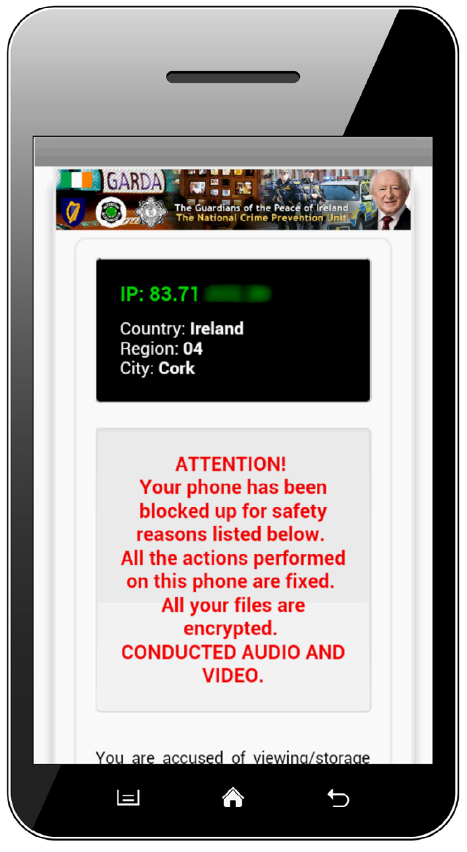
\includegraphics[width=0.48\textwidth]{img/android_locker.png}
  \end{center}
  \caption{Locker am Beispiel ``Lockdroid.G'' \cite{evolution}}
  \label{fig:lockdroid}
\end{wrapfigure}

Das Elaboration Likelihood Model geht davon aus, dass es zwei Wege zur Überzeugung gibt. Überzeugung durch die zentrale Verarbeitung der Mitteilung beschreibt die Abwägung und Qualität der Argumente. Hierbei wird also mit wohl überlegten Argumenten gearbeitet, um das Opfer zur Zahlung des Lösegelds zu bewegen. Im Falle von ``Lockdroid.G'' wäre das etwa die Tatsache, dass die Polizei das Smartphone ``aus Gründen der Sicherheit'' sperrt.\\
Die periphere Verarbeitung der Mitteilung beschreibt dagegen eher konditionierte Verhaltensweisen. Es wird davon ausgegangen, dass negativ oder positiv konnotierte Stichwörter zum Ergebnis führen. Als Beispiele hierfür kann z.B. das Logo der Polizei dienen oder auch die Anzeige des Landes, IP-Adresse und Stadt, die beim Opfer zur Angst führen, dass er etwas Illegales getan habe. \\

Wird noch angezeigt, dass der Nutzer illegal Dateien wie Musik oder Filme herunter geladen habe, führt dies dazu, dass er aus Angst vor sozialer Stigmatisierung nicht bei Bekannten oder der Polizei um Hilfe bittet.\\

Während Locker-Ransomware eher mit den psychologischen Faktoren innerhalb der Nachricht arbeitet, benutzt Crypto-Ransomware die Empfindungen den verschlüsselten Daten gegenüber und welchen Schaden das Opfer hätte, diese wertvollen Daten zu verlieren.\\

Zum einen enhalten viele Crypto-Ransomwares einen Countdown, nach dessen Ablauf die Daten endgültig verloren seien. Der Faktor Zeit wurde schon in Tests auf irrationale Entscheidungen hin untersucht. Zudem kann zum Countdown die Lösegeldforderung höher werden, je weiter die Zeit voran schreitet. Das setzt das Opfer so unter Druck, dass dieses bereitwillig bezahlt.\\
Das Ellsberg-Paradoxon der Entscheidungstheorie beschreibt das Verhalten von Menschen, die sich in einer Situation mit umgewissen Ausgang befinden. Wenn sie mit 2 Möglichkeiten konfrontiert sind, deren eine Möglichkeit einen Gewinn darstellt, dessen Wahrscheinlichkeit aber nicht abzusehen ist und der anderen Möglichkeit, dass sie etwas verlieren, aber dieser Verlust von der Wahrscheinlichkeit abzuschätzen ist, so nehmen Menschen eher den Verlust in Kauf.\\
Im Falle von Crypto-Ransomware haben die Menschen es mit zwei negativen Möglichkeiten zu tun: Einmal können sie nicht sicher sein, ob sie durch Bezahlung ihre Daten wieder erhalten. Auf der anderen Seite können sie noch weniger sicher sein, wieweit der Verlust ihrer Daten sie beeinflusst. Auch hier ist die Tendenz eher Richtung bezahlen und auf Wiedererhalt der Daten hoffen.

\begin{figure}[h!]
	\centering
	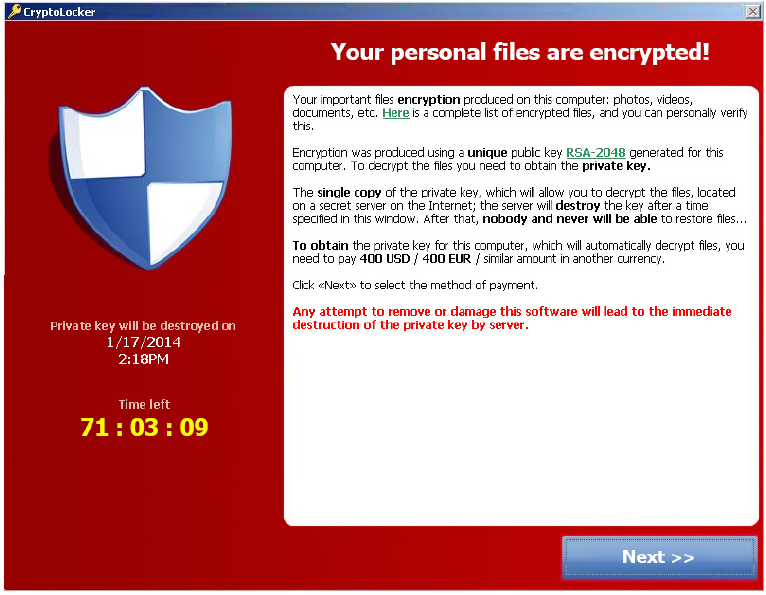
\includegraphics[width=\textwidth]{img/cryptolocker.png}
	\caption{Crypto-Ransomware am Beispiel ``Cryptolocker''\cite{evolution}}
	\label{fig:cryptolocker}
\end{figure}


\subsection{Preis und Bezahlsysteme}

Bereits die AIDS Ransomware hatte als Lösegeldsumme circa 300 \$ (Inflation eingerechnet), was dem Preis aktueller Ransomware entspricht\cite{evolution}.\\ 
Die durchschnittlichen Einkommen der unterschiedlichen Länder finden sogar Einzug in Ransomware: Um das Opfer zur Zahlung zu bewegen, darf sich die Lösegeldforderung nicht auf einem Level befinden, welches die Einkommensgrenze überschreitet. So wird in Ländern wie beispielsweise Indien oder Rumänien etwa ein anderer Betrag gefordert als in den USA und Deutschland. Technisch wird dies dadurch gelöst, dass sich ein infizierter Rechner bei dem Command-and-Control-Server der Angreifer meldet und dieser dadurch anhand der IP-Adresse eine grobe Zuordnung nach Ländern treffen kann.\\

Eine weitere Anpassung beim Preis wird bei der Unterscheidung zwischen Privatperson und Firma getätigt: Wird festgestellt, dass eine Firma betroffen ist, so werden einige Tausend Dollar verlangt, um die Daten zurückzuerhalten. Sicherheitsexperten haben heraus gefunden, dass der ideale Punkt, den Firmen noch bereit sind zu zahlen, und bei dem die Polizei noch keine Ermittlungen beginnt, bei 10.000 \$ liegt\cite{sweetspot}.\\

Um den Strafverfolgungsbehörden zu entgehen, ist es für die Ransomware-Community notwendig, anonym bezahlt zu werden, da sich so keine Spuren nachverfolgen lassen. War dies zur Zeiten von AIDS noch ein anonymes Postfach in Panama, so hat sich das im Digitalzeitalter geändert. Anfangs wurde noch der Anruf einer kostenpflichtigen Nummer oder die Bezahlung mit Bezahlgutscheinen wie Pasafecard oder CashU präferiert, inzwischen ist der Fokus bei Kryptowährungen wie Bitcoin. Diese ermöglichen es anonym zu bleiben und den Geldfluss nicht verfolgen zu können.\\

Interessant ist auch, dass je nach Ransomware-Art andere Bezahlsysteme zum Tragen kommen. Während durch Lockern der Rechner gesperrt ist, können etwa keine Bitcoins online gekauft werden, um mit diesen der Lösegeldforderung nachzukommen. In diesem Fall wird dann auf Bezahlgutscheine zurück gegriffen, die es einfach und schnell an vielen Tankstellen und Supermärkten zu kaufen gibt. Dagegen ist bei Crypto-Ransomware der Rechner noch bedienbar, also können noch Bitcoins erworben werden. Je nach Ransomware wird sogar ein Video als Anleitung dazu gezeigt.

\subsection{"`Probepackung"'}

Um dem Opfer zu demonstrieren, dass es die verschlüsselten Dateien wieder entschlüsselt bekommt, sollte es den Betrag bezahlen, bietet manche Ransomware an, dass eine handvoll zufällig ausgewählte Dateien des Rechners entschlüsselt werden. Dies steigert das Vertrauen der Opfer und erhöht die Chancen einer Bezahlung.

\section{Kryptographie}
\label{sec:sym_verschl}

Die symmetrische Verschlüsselung folgt dem Konzept, das sowohl für die Ver- als auch die Entschlüsselung jeweils die gleichen Schlüssel verwendet werden.

\begin{figure}[h!]
	\centering
	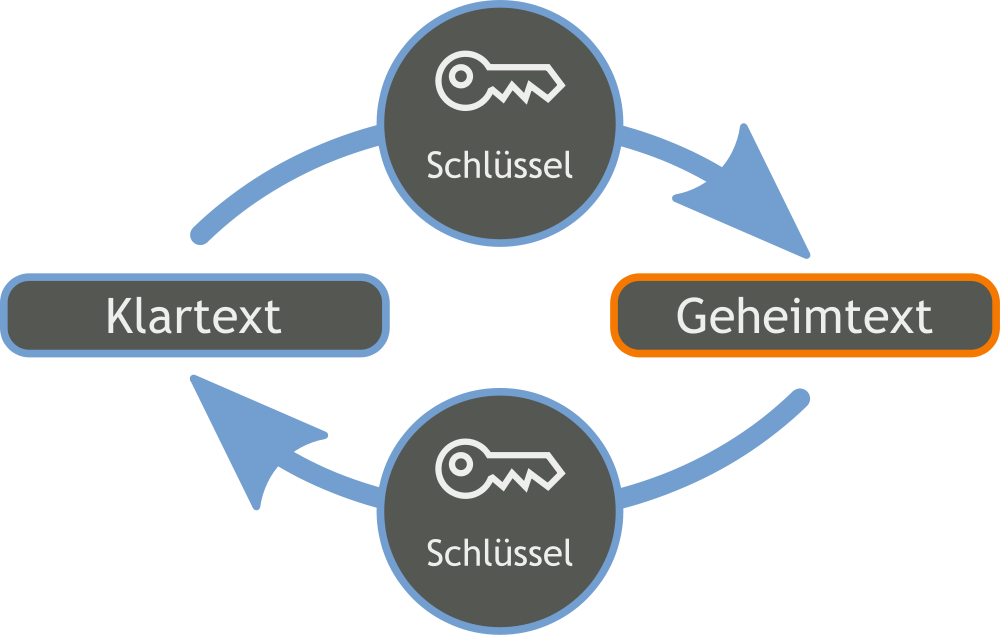
\includegraphics[scale=0.22]{img/SymKrypto.png}
	\caption{Symmetrische Verschlüsselung mit identischen Schlüsseln}
	\label{fig:sym_verschl}
	\end{figure}
	\footnotetext{Quelle: Bananenfalter (Public Domain) \\ \url{https://commons.wikimedia.org/wiki/File:Orange_blue_symmetric_cryptography_de.svg}}

Es gibt eine Reihe an unterschiedlichsten Algorithmen und Verfahren für symmetrische Verschlüsselung, allerdings hat sich mit \textsc{AES} ein Verfahren als de-facto Standard für verschiedenste Anwendungsbereiche etabliert.

AES ist hierbei eine Abkürzung für Advanced Encryption Standard und wird meist synonym für den Rijndael-Algorithmus verwendet. Dieses Verfahren ist heute so verbreitet, dass beispielsweise in modernen Prozessoren direkt als Maschinenbefehl zur Verfügung steht und somit deutlich größere Datenraten verarbeiten kann. \\
Benchmarks zeigen hier beispielshaft einen 6-fachen Speedup mit einer Datenrate von ca. 1.35 GB/s mit CPU-Unterstützung verglichen mit 212 MB/s ohne
CPU-Unterstützung.\footnote{aes:benchmark}

Vor allem durch die Hardware-Unterstützung ist es moderner Ransomware möglich, die CPU-Last während der Verschlüsselung derart in Grenzen zu halten, dass der Nutzer keine spürbare Langsamkeit des Systems bemerkt.


\subsection{Asymmetrische Verschlüsselung}
\label{sec:asym_verschl}

\begin{figure}[h!]
	\centering
	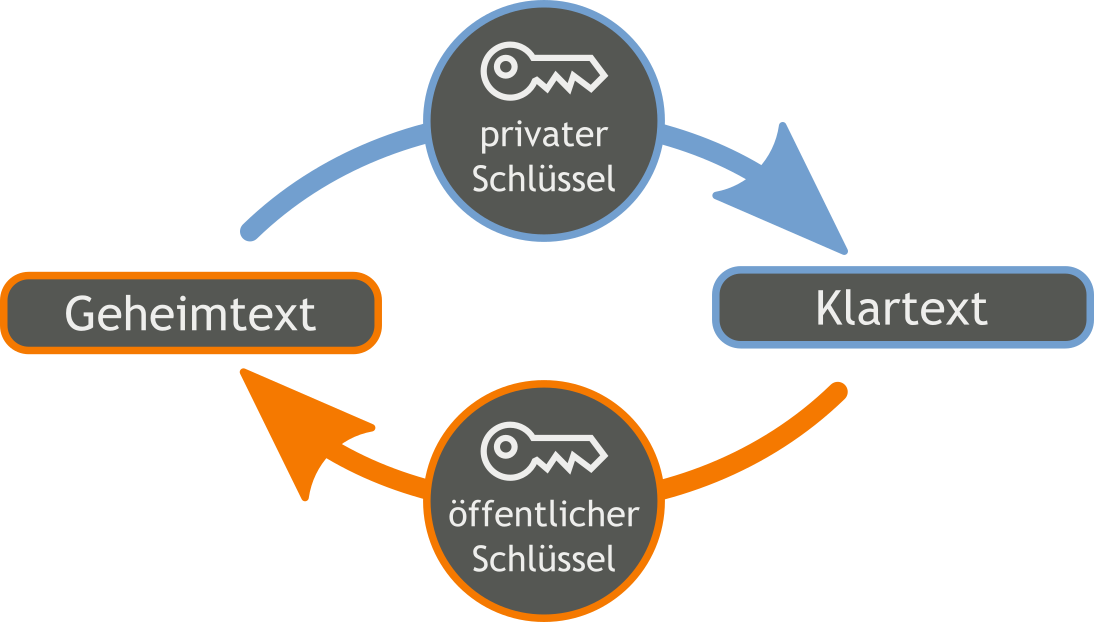
\includegraphics[scale=0.25]{img/AsymKrypto.png}
	\caption{Asymmetrische Verschlüsselung}
	\label{fig:asym_verschl}
	\end{figure}
	\footnotetext{Quelle: Bananenfalter (Public Domain) \\ \url{https://commons.wikimedia.org/wiki/File:Orange_blue_symmetric_cryptography_de.svg}} %TODO: Url


Asymmetrische Verschlüsselung basiert auf zwei Schlüsseln, einen öffentlichen und einen privaten. Diese Schlüssel gehören mathematisch zusammen und werden für unterschiedliche Zwecke verwendet.
Soll ein Klartext verschlüsselt werden, so wird hierfür der öffentliche Schlüssel des Empfängers verwendet. Die Entschlüsselung muss dann mit dem zugehörigen privaten Schlüssel erfolgen, eine Entschlüsselung mit dem öffentlichen Schlüssel ist nicht mehr möglich.

Auf Grund der Komplexität der Berechnungen ist das Verfahren langsam und auch nur schwer in Hardware abzubilden. Deshalb wird es nur für verhältnismäßig kurze Klartexte verwendet (< 1 KB), auch da die maximale Länge des Klartexts von der Länge des verwendeten Schlüssels abhängt. %TODO: Nachweis


Der große Vorteil von asymmetrischer Verschlüsselung liegt im sicheren Schlüsselaustausch, der nicht auf einen bereits gesicherten Kanal angewiesen ist, sondern auch über ein unsicheres Medium, beispielsweise über das Internet erfolgen kann, ohne dass es für einen Angreifer möglich ist die beteiligten Schlüssel zu belauschen oder zu berechnen. %TODO: MitM




\subsection{Hybride Verschlüsselung}
\label{sec:hybride_verschl}

Hybride Verschlüsselung kombiniert alle Vorteile von symmetrischer Verschlüsselung (Geschwindigkeit, Einfachheit) mit allen Vorteilen von asymmetrischer Verschlüsselung (Schlüsseltausch, Sicherheit).
Hierfür werden zufällige Schlüssel erzeugt, meist lange Zufallszahlen, die für die symmetrische Verschlüsselung verwendet werden. Diese Schlüssel werden Sitzungsschlüssel genannt und werden in der Regel nur einmalig verwendet (ein sog. One-Time-Pad). Nach der Verwendung werden die Sitzungsschlüssel asymmetrisch verschlüsselt und mit den codierten Daten zusammen übertragen.

Auf diese Weise lassen sich auch große Mengen an Daten effizient mittels asymmetrischer Kryptographie übertragen.


\section{Zahlung}
Test


\section{Tor}
Zur Absicherung der Kommunikation mit den Kontroll-Servern (C\&C-Server), die sowohl f�r 

\section{Prävention und Gegenmaßnahmen}
\subsection{Aktuelle Patchlevel}

	 Grundsätzlich sollte, um die allgemeine Sicherheit eines Systems zu verbessern, immer jegliche Software, sowohl des Betriebssystem wie auch die verwendete Anwendungssoftware, auf den aktuellen Stand gehalten werden. Ein besonders großes Risiko besteht bei Software, die zum öffnen von Inhalten aus den Internet verwendet werden, wie z.B. Web-Browser, Browser-Plugins, E-Mail-Programme, PDF-Betrachter und Büroanwendungen\cite{bsi:ransome}.\\
	 
	 Dies gilt in besonderem Maße für Systeme auf denen Windows betrieben wird, da diese für die Erpresser die größte Verbreitung ermöglichen, was der großen Verbreitung des Betriebssystems zuzuschreiben ist. Dies soll keinesfalls bedeuten, dass alternative Systeme weniger gefährdet sind, allerdings das Risiko bei Windows basierten Systemen erhöht sein könnte.
	 
\subsection{Angriffsfläche minimieren}

	Zudem kann die Angriffsfläche reduziert werden, indem nicht benötigt Software deinstalliert wird, wodurch auf die Anzahl der Software, die auf dem neuesten Stand gehalten werden muss sich verringert.\\
	
	Des Weiten ist kann das Systemweite deaktivieren der Script-Ausführung, wenn dies möglich ist das Risiko deutlich minderen, da Ransomware teilweise über E-Mail-Anhänge in Form von Javascript und VisualBasic-Skripten verteilt wird. Somit kann der Anhang nicht auf dem System ausgeführt werden und eine Infektion wird verhindert\cite{bsi:ransome}.\\
	
	Zudem ist es sinnvoll, wenn nicht benötigte Browser-Plugins deinstalliert werden (z.B. Flash, Java, Silverlight)\cite{bsi:ransome}\\, da diese bekanntermaßen häufig über Sicherheitslücken verfügen, was allein schon an den häufigen Sicherheits-Pachtes festgemacht werden kann.  
	
\subsection{Makros deaktivieren}

	Makros in z.B Excel können grundsätzlich ein Sicherheitsrisiko darstellen. Ransomeware kann sich z.B. unscheinbar wirkenden Excel, oder ähnlichen Dateien, als Makro verstecken. Bei aktuellen Office-Produkten ist das automatische ausführen von Makros zwar deaktiviert, in älteren allerdings nicht. Bei solch älterer Software ist es zudem häufig, dass diese nicht mehr mit Sicherheits-Updates versorgt werden, somit ist von der Verwendung sowieso abzuraten. 
	
\subsection{Text-Mail erzwingen}

	Dem BSI zufolge ist ist eine eine gute Idee, die HTML-Darstellung von E-Mails zu deaktivieren. Dies kann hilfreich sein, da für die Darstellung solcher E-Mails die selben Mechanismen benötigt werden, wie sie in Webbrowsern nötig sind. Dies bringt weiter Komplexität in die E-Mail Software und somit potentiell weitere Sicherheitslücken. Die können natürlich nicht ausgenutzt werden, wenn man entsprechende Komponente nicht nutzt. Zudem sollte man das automatische ausführen von Anhängen beim Anklicken verhindern\cite{bsi:ransome}.
	
	
\subsection{Greylisting / Tarpitting}
	
	Um einer Infektion durch Mail zuvorzukommen, hilft es den Angriffsvektor durch Empfang von Spam-Mails generell zu unterbinden. Die Erfahrungen der letzten Jahre haben gezeigt, dass Blacklisting generell eine schlechte Idee ist. Manche Blacklist-Dienste sperren gleich komplette Netzbereiche eines ISPs, wenn aus dessen IP-Adress-Bereich Spam verschickt wird. Greylisting ist eine 2003 erfundene Methode, die einen alternativen Ansatz bietet: Der empfangende Mail-Server schickt dem potenziellen Spammer eine Nachricht, dass der Service zurzeit überlastet ist und der Sender sich zu einem späteren Zeitpunkt nochmals melden soll. Dieses standardkonforme Verhalten aber wird von Spammern nicht implementiert und so melden sich nur reguläre Mail-Server nach einer Zeit wieder\cite{greylisting}. \\
	Einen Schritt weiter geht ``Tarpitting'', bei dem ähnlich wie bei der namensgebenden Teergrube die Geschwindigkeit verlangsamt wird. Der Spammer möchte soviel Mails wie möglich in kurzer Zeit versenden. Greylisting verjagt die Spammer zwar, aber lässt diese noch ungehindert ihr Werk tun. Die Tarpit reguliert den Mailempfang auf eine möglichst geringe Geschwindigkeit herunter, um so den Spammer möglichst lange im Sendezustand zu lassen. Solang diese Verbindung offen ist, wird er keine weitere öffnen. So wird beim Spammer eine Last erzeugt und dieser am massenhaften Versenden weiterer Mails gehindert.
	
\subsection{Serverseitige Mailfilter}

	
\subsection{Netzlaufwerke sichern}
\subsection{Netzwerke segmentieren}
\subsection{Zugänge sichern}
\subsection{Aktueller Virenschutz}

	Wie bereits beschrieben, benötigen die Antiviren-Hersteller circa 12 Stunden vom Zeitpunkt der Erkennung einer neuen Malware bis zum fertigen Update für ihre Softwarelösung. Um gegen eine Infizierung durch Ransomware gewappnet zu sein, ist es also anzuraten, möglichst täglich auf notwendige Updates hin zu überprüfen. Dies ist in nahezu allen Antiviren-Lösungen auch automatisch einstellbar.

\subsection{Nutzerschulung}

	Technische Lösungen sind immer nur ein Mittel zur Schadensbegrenzung, aber nie eine völlige Sicherheit vor Malware. Wie bereits dargelegt versucht Malware sich durch gefälsche E-Mails zu verbreiten, die dem Benutzer suggerieren, dass in einer angehängten Datei für ihn wichtiger Inhalt wäre. Zum Schutz vor Malware sollte hier den Benutzern eingeimpft werden, dass sie nur Anhänge von ihnen bekannten Personen öffnen. Nutzerschulungen sind leider kostspielig und müssen in regelmäßigen Abständen wiederholt werden, was der Grund ist, dass dies meist nicht stattfindet.


\subsection{Backups / Datensicherungen}

	Falls trotz aller getätigter Anstrengungen doch eine Infizierung erfolgte, ist es notwendig aktuelle Backups vorhanden zu haben. Diese sollten in regelmäßigen Abständen und automatisch erfolgen, da sie sonst erfahrungsgemäß irgendwann nicht mehr durchgeführt werden. Da Ransomware meist auch versucht auf Netzlaufwerke zuzugreifen, ist es wichtig, dass die Backups auf einem WORM-Medium (Write Once Read Many, etwa Bandspeicher) gespeichert werden. So kann verhindert werden, dass die Ransomware auch die Backups verschlüsselt.\\
	Ansonsten gilt wie üblich, dass Backups getestet werden müssen, um ihre Konsistenz und Wiederherstellbarkeit zu demonstrieren.
	
\subsection{Malwarebytes Anti-Ransomware}

	Das Computermagazin ``heise'' rät zur Installation der Software ``Anti-Ransomware'' der Firma Malwarebytes. Diese untersucht die laufenden Prozesse auf die typischen Merkmale von Ransomware, sprich es werden innerhalb kürzester Zeit Dateien verschlüsselt und mit einem neuen Namen versehen, der aus ursprünglichem Dateinamen und Ransomware-spezifischem Suffix besteht. Falls nun ein Prozess massenhaft Dateien umbenennen möchte, wird dies von ``Anti-Ransomware'' erkannt und dessen weitere Ausführung blockiert\cite{malwarebytes}.



\section{Zusammenfassung}
\subsection{Aktueller Stand}

\begin{table}[]
\centering
\label{ransom-table}
\caption{Aktueller Stand Ransomware}
\begin{tabular}{|l|l|}
\hline
\textbf{Ransomware} &                                                                                                                              \\ \hline
\textbf{}           &                                                                                                                              \\ \hline
Locky               & \cellcolor[HTML]{FFCC67}Necurs-Botnetz verschwunden.                                                                         \\ \hline
KeyRanger           & \cellcolor[HTML]{9AFF99}Neuinstallationen von Apple verhindert.                                                              \\ \hline
Petya               & \cellcolor[HTML]{FFCC67}Daten-Wiederherstellung möglich.                                                                     \\ \hline
TeslaCrypt          & \cellcolor[HTML]{9AFF99}\begin{tabular}[c]{@{}l@{}}Entwicklung eingestellt.\\ Daten-Wiederherstellung möglich.\end{tabular}  \\ \hline
CryptoLocker        & \cellcolor[HTML]{9AFF99}\begin{tabular}[c]{@{}l@{}}ZeuS-Botnetz zerschlagen.\\ Daten-Wiederherstellung möglich.\end{tabular} \\ \hline
\end{tabular}
\end{table}

Die Sicherheitsbestrebungen der IT-Security-Dienstleister haben soweit Erfolg gezeigt und aktuelle Varianten von Ransomware konnte so Einhalt geboten werden. Aber nicht nur von Seiten der Computerindustrie wird versucht Ransomware zu stoppen, auch die Strafverfolgungsbehörden machen den Entwicklern zunehmend das Leben schwer: Durch die Festnahme von 50 russischen Hackern, so wird vermuted, wurde eines der größten Botnetze der Welt zum Stillstand gebracht\cite{angler}.

\subsection{Zukunft}

Die aktuelle Flut an Ransomware ist soweit es geht eingedämmt, wobei es hier nur eine Frage der Zeit ist, bis sich neue Varianten entwickeln und verbreiten. Noch keine Malware hatte den gleichen monetären Erfolg wie Ransomware zurzeit. Durch das Internet of Things (IoT) wird es immer mehr Geräte geben, die anfällig für Ransomware sind, vor allem in Anbetracht der Tatsache, dass die Hersteller von IoT-Geräten oftmals aus Geschäftsbereichen kommen, die mit IT und IT-Sicherheit noch keinen Kontakt hatten. Diese Firmen haben noch keine Erfahrungen mit Sicherheitslücken gemacht und werden höchstwahrscheinlich, sobald ihre Produkte auf dem Markt sind, auch keine Updates heraus bringen.\\
Wie in ``The Evolution Of Ransomware'' bereits angemerkt ist, werden sich die Angreifer weiter nicht nur mit Computer und Handys als Ziele beschäftigen, sondern auch andere verheißungsvolle Bereiche suchen. Mitte Juni 2016 wurde bekannt, dass die erste Ransomware für Smart-TVs entdeckt wurde\cite{smarttv}.


%\subsubsection*{Acknowledgments}


%%%%%%%%%%%%%%%%%%%%%%%%%%%%%%%%%%%%%%%%%%%%%%%%%%%%%%%%%%%%%%%%%%%%%%%%%%%%%%%
\newpage
\bibliographystyle{splncs03}
\bibliography{paper}
%%%%%%%%%%%%%%%%%%%%%%%%%%%%%%%%%%%%%%%%%%%%%%%%%%%%%%%%%%%%%%%%%%%%%%%%%%%%%%%

\end{document}
